\Section{Feature-based Testing of Mobile Apps}
\label{framework}

%Our bug study revealed a number of bug categories that correspond to user-interaction features possible with mobile devices. These features are independent of the logic but tied to GUI states of apps. Such features are present in most mobile apps and there is a common understanding of how an app should support a feature. According to the bug study, examples of features are rotation, activity life-cycle transitions, and gestures. We can identify more features like Android Back button as possible sources of bugs not present in the bug study.

% DECLARE: We describe how to test user-interaction features of mobile apps
The findings of our bug study motivated us to develop an approach for automatically testing user-interaction features (interaction features, or simply features for short throughout the paper) of mobile apps. Our proposed approach is described in this section. We start by defining some terminology.

% PRELIMINARIES
% PRELIMINARIES OF FRAMEWORK SECTION: Currently not a separate sub-section

% Define interaction features
\begin{mydef}[Interaction feature]
\label{def:interactionFeature}
An interaction feature is an action supported by the mobile platform, which enables a human user to interact with a mobile app, using the mobile device and the graphical user-interface (GUI) of the app. Further, an interaction feature is associated with a common sense expectation of how the mobile app should respond to that action. 
\end{mydef}
\vspace*{-2ex}

% Natural language explanation of user-interaction features
Interaction features include actions like rotating a mobile device, general purpose gestures like zooming in/out or scrolling, and actions which start, pause, kill or resume operation of an app, taking its Activity GUI components through various states in their life-cycle. These features were discussed in our bug study. In addition, features like the \textit{Back} or \textit{Up} buttons of the Android platform\footnote{See \url{http://developer.android.com/design/patterns/navigation.html}.} are also valid interaction features. Note that the above definition \textit{excludes} a number of common gestures such as {\small\texttt{click}} or {\small\texttt{longClick}}, or other custom gestures, for which there is no standard expected response from apps; it is completely context and application specific. Since a given interaction feature will have, in general, a standard expected behavior, across apps and different mobile platforms\footnote{Specific apps may of course choose to modify this standard response.}, this provides a general, app agnostic \textit{oracle} for validating an app's response to exercising that feature. Thus, a key component of our approach is authoring such reusable oracles and employing them in interaction feature testing.

% GUI Model and GUI States
We follow a model-driven approach to generating test-cases for testing interaction features of a given mobile app. The starting point for our technique is a finite state model of the GUI behavior of the app, which is defined as follows.

\begin{mydef}[GUI model]
\label{def:GUImodel}
A GUI model of an app is a finite state machine $\mathcal{M}$, denoted by the $4$-tuple $\mathcal{M} = (S, s_0, A, R)$, where $S$ is a finite set of abstract states representing different GUI screens, $s_0 \in S$ is the initial state denoting the app's opening screen, $A$ is a finite set of application specific actions the user may perform in executing the logic of the app, and $R \subseteq S \times A \times S$ is a transition relation describing transitions between states in $S$ in response to user actions from $A$.  
\end{mydef} 
\vspace*{-2ex}

%%%%% INCORPORATE THESE POINTS BELOW
%We identify the following properties for user-interaction features (features for short throughout the paper).
%\begin{itemize}
%\item 
%(1) A user-interaction feature is a way of interacting with the mobile device at the GUI level that is common between apps.
%\item 
%(2) There is an app agnostic \emph{oracle} for a feature. Even though it is possible to redefine how an app responds to exercising a feature, there is a common sense of what should happen in most apps.
%\item 
%(3) In most cases, features are so app agnostic that they are not explicitly included in GUI models. For instance, what happens after killing or pausing an app is rarely included in the GUI model and is usually inferred from the activity life-cycle.
%\item 
%(4) Even though features are usually absent from GUI models, apps have to actually implement feature functionalities and are expected to support features and give the results anticipated by features' oracles.
%\end{itemize}

% Further explanation of GUI Models, GUI models as directed graphs
Two GUI screens are represented by the same abstract state in
$\mathcal{M}$ if and only if they contain the same set of actions on
the same widgets. The only exception to this is screens showing
collections of items, such as books, files, songs, transactions,
\textit{etc.}, where each item supports some set of actions. In this
case two screens with different (non-zero) numbers of items are
interpreted as the same state. Thus, the contents of a collection are
abstracted as empty or non-empty.  Similar notions of GUI states have
also been used in previous work~\cite{Dynodroid:2013,
  collider2013}. The set $A$ includes application specific actions
such as clicks or longClicks, \textit{etc.,} on specific widgets but
\textit{does not} include platform supported interaction features (e.g., device rotation, \textit{etc.}). We
believe this is typical of GUI models as well~\cite{YangFASE2013}.

Note that although the visible part of a GUI screen of a mobile app, as viewed on a mobile device, may change by performing an action such as a device rotation, a zoom, or a scrolling action, these apparently different screens still correspond to the same abstract state in the GUI model. We define the notion of a \textit{view}, denoted by the symbols $w$, to represent the visible portion of abstract GUI model states $s$. Thus, a state $s$ can have several views, generated by exercising different available interaction features on $s$. Specifically, we use the notation $\Phi(s, \mathbf{u}, -)$ and $\Phi(s, \mathbf{u}, +)$ to denote respectively, the two different views of state $s$ before and after action (or action sequence) $\mathbf{u}$ was fired, where $\mathbf{u}$ corresponds to an instance of exercising an interaction feature. The view notation provides a relative notion of \textit{time} of sampling states (for their current view), before and after exercising interaction features.

A GUI model $\mathcal{M}(S, s_0, A, R)$ can also be represented as a rooted, labeled directed graph $G = \langle V, E, r, A, \mathcal{L} \rangle$, in a straightforward manner. Here, the nodes $V$ represent the states $S$, the root node $r$ represents initial state $s_0$, edges $E$ represent transitions between states, consistent with transition relation $R$, and the labeling function $\mathcal{L} \colon E \to A$ labels each edge with the action $a \in A$ responsible for the transition. GUI models can either be constructed manually or generated automatically using one of the techniques from a growing body of work on GUI model generation for mobile apps~\cite{AmalfitanoASE2012, Joorabchi:2012:WCRE, YangFASE2013}.
%to automatically generate tests that exercise features and assert oracles.

% Summarize Overall Approach
\textbf{Overall Approach:} 
Our technique generates compact test suites, complete with test oracles, to comprehensively test interaction features of a given mobile app. The approach uses an extensible library $\mathcal{F}$ of reusable and application agnostic feature definitions, described in Section~\ref{sec:featureDefinition}. Given a user provided GUI model of the app we automatically augment this model with feature instances, using the feature definitions in $\mathcal{F}$ (Section~\ref{sec:modelAugmentation}). %using user feedback to customize the features when needed. 
Then, based on the cost and test adequacy criteria defined in Section~\ref{sec:testSuiteDefinition}, we automatically traverse the augmented model to create compact test sequences (Section~\ref{sec:traversalAlgo}). Finally, we automatically instantiate test oracles in the test sequences to obtain a compact and complete test suite.
%a complete test suite that tests the user-interaction features of the app. 



% FORMAL DEFN. OF FEATURE & EXAMPLES
\Subsection{Authoring Oracles for Interaction Feature Testing}
\label{sec:featureDefinition}

We introduce an extensible framework in which interaction features can be defined in an application agnostic manner and stored in a library. When testing a given app our technique appropriately instantiates features from the library, using these feature definitions, and generates tests, complete with test oracles, to comprehensively test each feature.

\begin{mydef}[Feature definition]
\label{def:feature}
The feature definition of a given interaction feature $f$ is a triple: $\langle \mathbf{u}_f, D_f(s), O_f(w_1, w_2) \rangle$. %we need the following triple: $\langle S_f, A_f, O_f(s_1, s_2, \ldots, s_k) \rangle$. $S_f \subset S$ is a subset of the app's GUI states on which the feature is applicable.
$\mathbf{u}_f = \langle u_1, u_2, \dots, u_n \rangle$ is a sequence of actions that exercises the feature. $D_f(s)$ is the destination function, that maps a given state $s$ at which the feature can be exercised to a set of states $S_f \subseteq S$ that could potentially result from exercising $f$ at state $s$. $O_f(w_1, w_2)$ is the oracle for feature $f$, where $w_1 = \Phi(s_1, \mathbf{u}_f, -)$ is a view of some state $s_1$
before firing actions $\mathbf{u}_f$ and $w_2=\Phi(s_2, \mathbf{u}_f, +)$ is a view of a state $s_2$ reached after firing actions $\mathbf{u}_f$ on some previous state $s_1$, possibly the same state $s_2$.
%$O_f(s_1, s_2, \ldots, s_k)$ is the oracle for feature $f$. It is a boolean predicate over the set of states $s_1, s_2, \ldots, s_k \in S$ which evaluates to \texttt{true} if states $s_1, s_2, \ldots, s_k$ satisfy the specific relationship encoded in the predicate, and \texttt{false} otherwise.
\end{mydef}
\vspace*{-2ex}

A crucial aspect of the above feature definition is to express $\mathbf{u}_f$, $D_f$, and $O_f$ in an application agnostic manner. We demonstrate how to do this below, through example feature definitions of several common interaction features. Another important restriction implied by Definition~\ref{def:feature} is that the set of abstract states in the GUI model should be closed under application of the interaction feature, \ie exercising the feature in one of the states should not take the application to a fundamentally new abstract state outside the GUI model. This common sense restriction is also valid for all interaction features in our knowledge. In the following examples we use $\Phi^-(s)$ and $\Phi^+(s)$ as shorthand for $\Phi(s, \mathbf{u}_f, -)$ and $\Phi(s, \mathbf{u}_f, +)$ respectively, since $\mathbf{u}_f$ is clear from the context.

%In many if not most practical instances, fully automatable oracles typically involve a predicate over two states. For example, the oracle for a double screen rotation\footnote{Rotating the screen $90^\circ$ twice consecutively.} would assert that the application GUI states $s_1$ and $s_2$ that exist before and after the double rotation should be equal, i.e., $(s_1 = s_2)$.

%We introduce an extensible language for defining features oracles ($O_f$'s). One can add to the set of features by identifying the relationship between the expected state and an existing state. For some user-interaction features, the expected state after exercising the feature is exactly the same as a previously seen state. Examples of such features are as follows.

{\bf Double rotation (DR):} We incorporate the mobile device rotation feature in a \textit{double rotation} feature definition, which expresses the act of rotating a mobile device and then rotating it back to the original orientation. With this action the application should stay in the same state. Further, the view of that state before an after double rotation should be identical. This is expressed in the feature definition: $\mathit{DR} = \langle \mathbf{u}_f = \langle rotate, rotate\rangle, D_f(s) = \{s \}, O_f = (\Phi^-(s) = \Phi^+(s)) \rangle$.
%O_f = (\Phi(s, \mathbf{u}_f, -) = \Phi(s, \mathbf{u}_f, +)) \rangle$.
\\
\indent
{\bf Killing and restarting (KR):} The operating system might choose to kill and then restart an app for various reasons (\eg low memory). Similar to double rotation, the app should retrieve its original state and view. Thus, $ \mathit{KR} = \langle \mathbf{u}_f = \langle kill, restart\rangle, D_f(s) = \{s \}, O_f = (\Phi^-(s) = \Phi^+(s)) \rangle$.
\\
\indent
{\bf Pausing and resuming (PR):} The app can be paused (\eg by hitting the Android Home button) and then resumed. $ \mathit{PR} = \langle \mathbf{u}_f = \langle pause, resume\rangle, D_f(s) = \{s \}, O_f = (\Phi^-(s) = \Phi^+(s)) \rangle$. Killing and then restarting, and pausing and then resuming are both instances of activity life-cycle transitions which all apps should support.
\\
\indent
{\bf Back button functionality (Back):} The Back button is a hardware button on Android devices which takes the app to the previous screen. $ \mathit{Back} = \langle \mathbf{u}_f = \langle back \rangle, D_f(s) = \{s_p : s_p \in parent(s) \}, O_f = (\Phi^-(s_1) = \Phi^+(s_1)) \rangle$, where $s_1 \in D_f(s)$. In this case, the destination function produces a set of destinations $D(s)$ corresponding to each of the parent (using the standard graph theoretic notion of parent and child) nodes of the current state $s$ in the GUI model.
\\
%$\langle S_f = S, A_f = \langle a_1, back\rangle, O_f = (s_1 = s_2)\rangle$ where $a_1$ is any navigation action in the app model that takes the app from one screen to another.
\indent
{\bf Opening and closing menus (Menu):} The hardware Menu button on Android devices opens and closes custom menus that each app defines. For this feature definition $\mathit{Menu} = \langle \mathbf{u}_f = \langle menu, menu\rangle, D_f(s) = \{s \}, O_f = (\Phi^-(s) = \Phi^+(s)) \rangle$.

%{\bf Up functionality:} The Up button was introduced in Android 3.0. It appears on the top left corner of the screen and consists of the app icon and a left-point caret. The Up functionality is similar to Back, except that Back always takes the app to the previous screen while Up takes it to the parent screen, which might or might not be the same. As opposed to Back, the model has to define the target of the Up functionality, since it is not uniquely defined and depends on how the hierarchy of screens is viewed. If $s_1$ and $s_2$ are the states before and after hitting the Up icon and $s_3$ is the expected target of Up after $s_1$ according to the model then we have $\langle S_f = S - \{top\}, A_f = \langle up\rangle, O_f = (s_3 = s_2)\rangle$. $top$ is the topmost level screen for which Up is undefined.

%{\bf Double scrolling:} Scrolling down and then back up should bring back the original screen. $\langle S_f = S, A_f = \langle scrollDown, scrollUp\rangle, O_f = (s_1 = s_2)\rangle$.

In the above instances the oracle was always an assertion of equality between two appropriate state views. In general, however, the oracle predicate can include arbitrary relational or logical operators. %For some other user-interaction features, the expected state is a subset or a superset of a previously seen state.
For example:

{\bf Zooming in (ZI):} Zooming into a screen should bring up a subset of what was originally on the screen. $\mathit{ZI} = \langle \mathbf{u}_f = \langle zoomIn\rangle, D_f(s) = \{s \}, O_f = (\Phi^-(s) \supset \Phi^+(s)) \rangle$.
\\
\indent
{\bf Zooming out (ZO):} Zooming out from a screen should result in a superset of the original screen. $\mathit{ZO} = \langle \mathbf{u}_f = \langle zoomOut\rangle, D_f(s) = \{s \}, O_f = (\Phi^-(s) \subset \Phi^+(s)) \rangle$.
\\
%The user can extend the set of user-interaction features by defining new oracles. For instance:
\indent
{\bf Scrolling (SCR):} Scrolling down (or up) should display a screen that shares parts of the previous screen. $\mathit{SCR} = \langle \mathbf{u}_f = \langle scrollDown\rangle, D_f(s) = \{s \}, O_f = (\Phi^-(s) \cap \Phi^+(s) \neq \emptyset) \rangle$.
%$\langle S_f = S, A_f = \langle scrollDown\rangle, O_f = (s_1 \cap s_2 = \emptyset (or \neq \emptyset)))\rangle$.
%Previous work \remark{ref?} showed bugs that would make the app run out of memory in case of many scrolls.

Note that the feature definition itself includes an implementation of the oracle, albeit an app independent one, that can be re-used across different apps. Thus, the semantics of operators used in the oracles are defined there.


% GUI MODEL AUGMENTATION USING FEATURE LIBRARY
\subsection{Augmenting GUI Models with Feature Instantiations}
\label{sec:modelAugmentation}

Given a GUI model $G = \langle V, E, r, A, \mathcal{L} \rangle$ of the target app and a library $\mathcal{F}$ of interaction features, specified as discussed in Section~\ref{sec:featureDefinition}, the next step in our approach is to annotate $G$ with all possible instantiations of each feature in $\mathcal{F}$ to produce an augmented GUI model $G^+ = \langle V, E^+, r, A^+, \mathcal{L}^+ \rangle$. Specifically, this involves adding a set of special labeled edges, called \textit{golden edges}, to $G$. Each golden edge, $e_f(v_1, v_2)$ denotes that feature $f$ when exercised at the state of vertex $v_1$ takes the application to the state of vertex $v_2$. Further, $e_f$ is labeled with $\mathbf{u}_f$, the action sequence of feature $f$. Thus, the augmented model $G^+$ includes the augmented set of edges $E^+ = E \cup E_{golden}$,  augmented action set $A^+ = A \cup \bigcup_{f \in \mathcal{F}} \mathbf{u}_f$, and appropriately modified labeling function $\mathcal{L}^+: A^+ \rightarrow E^+$, where $E_{golden}$ are the golden edges and $\bigcup_{f \in \mathcal{F}} \mathbf{u}_f$ are the actions for features $\mathcal{F}$ labeling the golden edges.

\begin{algorithm}[t]
\begin{footnotesize}
  \DontPrintSemicolon
  \SetAlFnt{\scriptsize\scriptfont}
  \SetKwData{Left}{left}\SetKwData{This}{this}\SetKwData{Up}{up}
  \SetKwFunction{Union}{Union}\SetKwFunction{FindCompress}{FindCompress}
  \SetKwInOut{Input}{Input}\SetKwInOut{Output}{Output}
  \caption{GUI Model Augmentation Algorithm}\label{alg:augmentGUImodel}
  \Input{$G = \langle V, E, r, A, \mathcal{L} \rangle$: Original GUI model of target app \\
  	$\mathcal{F}$: Feature library
  }
  \Output{$G^+ = \langle V, E^+, r, A^+, \mathcal{L}^+ \rangle$: Augmented GUI model}
  \BlankLine
  \Begin{
  		$G^+ \leftarrow G$\;
  		\ForEach{$v \in V$}{
  			\tcp{Iterate over each vertex (state) of $G$}
  			\ForEach{$f \in \mathcal{F}$}{
  				\tcp{Iterate over each feature in $\mathcal{F}$}
  				$dSet = \mathit{destinationSet}(v, G^+, f) $\;
  				\ForEach{$v_1 \in dSet$}{
  					$e \leftarrow \mathit{createEdge}(v, v_1);$\;
  					$\mathit{setEdgeLabel}(e, getAction(f))$\;
  					$\mathit{markGolden}(e)$\;
  					$\mathit{addEdge}(e, G^+)$\;
  				}
  			}
  		}
			\Return{$G^+$}\;
  }
\end{footnotesize}  
\end{algorithm}

Algorithm~\ref{alg:augmentGUImodel} shows the procedure to perform GUI model augmentation. The algorithm iterates over each state $v$ in the GUI model (lines $3-13$) and each feature $f$ in library $\mathcal{F}$, instantiating $f$ at $v$, as per the feature definition. It computes the set of possible destination vertices $dSet$, by evaluating function $D_f$ in the feature definition (function $\mathit{destinationSet()}$ on line $5$). It then iterates over each possible destination vertex $v_1$ (lines $6-11$) creating and adding a golden edge, labeled by the feature's action sequence $\mathbf{u}_f$ (line $8$), to the augmented model $G^+$.
Figure~\ref{fig:dotGraph} shows the GUI model of our simplified version of Kitchen Timer from Section~\ref{example}, augmented with golden edges for the Double Rotation and Back button features.

\begin{figure*}[!t]
\centering
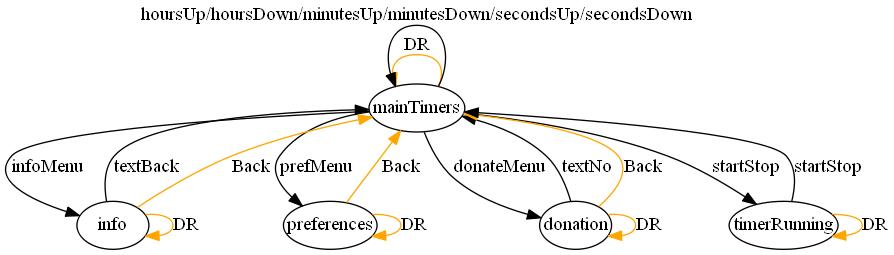
\includegraphics[width=0.65\textwidth]{figures/dotGraph.jpg}
\caption{Simplified Model of Kitchen Timer.}
\label{fig:dotGraph}
\end{figure*}


% TEST SUITE DEFINITION (test case, covering features through test cases, test-suite cost function)
\subsection{Test Suite Definition}
\label{sec:testSuiteDefinition}

Given an augmented GUI model $G^+$ the final phase of our technique generates a test suite with the following goal.

\noindent\textbf{Test objective:} \textit{A \textbf{compact} suite of tests to \textbf{comprehensively} test the interaction features of the given app under test.}

 A test is a sequence of actions (\ie a sequence of edges or a path in $G^+$) starting at the initial state $r$, with each action possibly followed by an oracle check. Therefore, a test can be represented as $\langle a_1, o_1, \dots, a_n, o_n \rangle$. Each $a_i \in A^+$ is any action (including those that exercise interaction features) allowed by the app's GUI. Each $o_i$ is either an oracle check or no operation. We assume that oracle checks are side effect free, \ie they do not change the state of the app.

We define a test adequacy criterion to concretize the notion of a ``comprehensive" test suite stated in the test objective. Since mobile apps are event-driven systems and interaction features are elements of the app's GUI, we develop a criterion that is motivated by the notions of path coverage and event-flow coverage used by previous work on GUI testing~\cite{memon2001coverage}. This is in contrast to code coverage-based criteria such as line or branch coverage, which would be more appropriate for functional testing of the software implementation rather than testing its high level platform features, as in our case. Intuitively, we say that a test suite covers a feature, if it contains tests to exercise and validate \textit{each possible instance} of exercising that feature on that app. Simply put, this implies exercising the feature in each GUI state. Given a test suite $T$, an interaction feature $f$ from a feature library $\mathcal{F}$ and an augmented GUI model $G^+ = \langle V, E^+, r, A^+, \mathcal{L}^+ \rangle$, as defined in Section~\ref{sec:modelAugmentation}, we define adequacy of $T$ in testing $f$ with respect to $G^+$ as follows.

\begin{mydef}[Interaction feature coverage]
\label{def:coverage}
A test suite $T$ covers a feature $f$ iff $\forall s \in S: \exists t \in T, t = \langle a_1, o_1, \dots, a_n, o_n  \rangle, \exists j, k, 0 \leq j < k \leq n$ such that $\langle a_1, \dots, a_j \rangle$ takes the app from the initial state $s_0$ to state $s$, $\langle a_{j+1}, \dots, a_k \rangle = \mathbf{u}_f$, and $o_k = O_f$.
\end{mydef}

Since there are no standard or widely accepted cost functions to optimize test suites we quantify the ``compactness"  of our test suite using the common sense observation that large test suites are hard to set up, execute, and maintain. The size of a test suite can be measured by the number of tests it contains as well as the cumulative number of operations (actions $a_i$) in the test suite as a whole.
We propose a customizable cost function that captures this.

%intuitively measures the time it takes to execute a test suite, including the set up and execution times. 
%Then we show how to leverage this cost function to traverse the model more effectively, in order to get smaller and faster to run test suites.

\begin{mydef}[Cost of a test suite]
\label{def:costfunction}
The cost of a test suite T is $cost(T) = \alpha * |T| + \beta * \Sigma_{t \in T} |t|$, where $\alpha$ and $\beta$ are positive co-efficients. \end{mydef}

Coefficient $\alpha$ measures the relative cost of developing and maintaining a suite, which scales with the number of tests in a suite. Coefficient $\beta$ quantifies the cost of executing actions and asserting oracles which is proportional to the number of operations.


% TEST SUITE GENERATION
\Subsection{Feature-based Test Sequence Generation}
\label{sec:traversalAlgo}

Recall that interaction features are orthogonal to the core logic of the app and their function is typically to help the user navigate or access content on the app by mutating the state of the app's GUI. Further, exercising an interaction feature on a given state has no side effects in terms of the GUI model, \ie the effect of exercising that feature is limited to a single GUI screen and has no impact on the downstream actions. This observation is very important as it allows us to arbitrarily mix and match instances of several features (and their test oracles) in a single test case, as long as it lowers the cost of the test suite, per Definition~\ref{def:costfunction}. Since each instance of every feature is already recorded in our augmented GUI model $G^+$ (servicing the test adequacy criterion of Definition~\ref{def:coverage}), our test generation problem can be stated as follows.

\noindent\textbf{Test suite generation problem:} \textit{Given an augmented GUI model $G^+$ generate a minimum cost test suite such that each golden edge in $G^+$ is covered by at least one test in the suite.}

%\begin{proof}
%The proof sketch is by reducing the \textit{minimum path cover problem}~\cite{PathCover:NtafosH79} to this problem as follows. Given an instance of the minimum path cover problem, take the given directed graph $G$ and construct a modified $G'$ from it:
%\begin{enumerate}
%\item Add a self loop to every vertex and mark it as golden (ensuring that we cover all golden edges if and only if we cover all vertices).
%\item Add a new root node $r$ and add an edge from $r$ to each vertex of $G$ (accounting for the fact that in the original path cover problem paths need not originate at a starting node, which they do in our case).
%\end{enumerate}
%Now we solve our problem on $G'$ with $\alpha = 1$ and $\beta = 0$, thus minimizing the number of $r$-originating paths covering all golden edges, or essentially all vertices, irrespective of path lengths. The answer would be a minimum path cover over $G$.
%\end{proof}

It can be shown that the above problem is NP-hard, by reducing the \textit{minimum path cover problem}~\cite{PathCover:NtafosH79} to this problem. We omit the detailed proof here for lack of space.

We propose a greedy algorithm for this NP-hard problem. In addition, we introduce two optimizations to further reduce the cost associated with covering features. Algorithm~\ref{alg:traversalAlgo} shows a pseudo-code of the traversal algorithm we propose. The input to this algorithm is the augmented graph model. We use a set to keep track of \emph{covered edges} $CE$ and a stack to record the test sequence. First, on Line~\ref{line:BFS}, we sort the nodes based on their increasing distance from the root using a Breadth First Search (BFS) and keep the sorted list in $L$. For example, we can sort the nodes of Figure~\ref{fig:dotGraph} as $\langle$\emph{mainTimers}, \emph{info}, \emph{preferences}, \emph{donation}, \emph{timerRunning}$\rangle$. Then, working through the list $L$ on Line~\ref{line:loopForL}, we select the next node $s$ that has uncovered outgoing edges (Line~\ref{line:sHasOutgoing}). In our example, the first node in the list with uncovered outgoing edges is \emph{mainTimers} (as we have not yet covered any edges). We use the shortest path from the root to this node (saved through previously performed BFS) as the prefix of all sequences to be generated starting from it. Lines~\ref{line:prefixBeg} to \ref{line:prefixEnd} iterate through the shortest path and (1) mark edges as visited by adding them to $CE$, and (2) push them onto $stack$. The rationale behind using such a prefix is to minimize the cost associated with taking edges to get to a given node, where the exploration for uncovered golden edges begins. % In the case of \emph{mainTimers}, the prefix would be empty as \emph{mainTimers} is the root of the graph.

%\lstinputlisting[caption=Traversal Algorithm in Java.,label=lst:traversalAlgo]{listings/traversalAlgo.java}
\begin{algorithm}[t]
\begin{footnotesize}
  \DontPrintSemicolon
  \SetAlFnt{\scriptsize\scriptfont}  
  \SetKwData{Left}{left}\SetKwData{This}{this}\SetKwData{Up}{up}
  \SetKwFunction{Union}{Union}\SetKwFunction{FindCompress}{FindCompress}
  \SetKwInOut{Input}{Input}\SetKwInOut{Output}{Output}  
  \caption{Traversal Algorithm}\label{alg:traversalAlgo}
  \Input{$G^+ = \langle V, E^+, r, A^+, \mathcal{L}^+ \rangle$: Augmented GUI model of app}
  \Output{$T$: Test Suite}
  \BlankLine
  \Begin{
  		$CE \leftarrow \emptyset$\;
  		$stack \leftarrow \emptyset$\;
  		$L \leftarrow \mathit{sortWithBFS}(G^+)$\;\nllabel{line:BFS}
  		\ForEach{$s \in L$}{\nllabel{line:loopForL}
  			\While{$\exists (s,y) \in outGoing(s), s.t. (s,y) \in E-CE$}{\nllabel{line:sHasOutgoing}
  				\ForEach{$e \in shortestPathBFS(r,s)$}{\nllabel{line:prefixBeg}
  					$stack.push(e)$\;
  					$CE \leftarrow CE \cup \{e\}$\;
  				}\nllabel{line:prefixEnd}
  				$c \leftarrow s$\;
  				$stop \leftarrow false$\;
  				\While{$!stop$}{\nllabel{line:loopForTraversalBeg}
  					\If{$\exists (c,v) \in outGoing(c), s.t. (c,v) \in E-CE$}{\nllabel{line:cHasOutgoing}
  						$CE \leftarrow CE \cup \{(c,v)\}$\;\nllabel{line:coverIt}
  						$stack.push((c,v))$\;\nllabel{line:pushIt}
  						$c \leftarrow v$\;\nllabel{line:updateC}
  					}\lElse{$stop \leftarrow true$\;\nllabel{line:stopToTrue}}
  				}\nllabel{line:loopForTraversalEnd}
  				$T \leftarrow T \cup stack$\;
  				$stack.clear()$\;
  			}
  		}
  		\Return{$T$}\;
	}
\end{footnotesize}  
\end{algorithm}

Then, using $c$ as a pointer to the \emph{current} node, which is initially set to $s$, on Line~\ref{line:cHasOutgoing} we pick an uncovered edge going out of $c$. We take this edge, mark it as covered (Line~\ref{line:coverIt}), push it onto $stack$ (Line~\ref{line:pushIt}), and update $c$ to the destination of this edge accordingly (Line~\ref{line:updateC}). Once we get to a node that has no uncovered outgoing edge, the current test sequence is complete and we set $stop$ to {\small\texttt{True}} on Line~\ref{line:stopToTrue}. The current $stack$ makes one test sequence and we continue by generating more sequences and adding them to $T$ which is the test suite and is the output of this algorithm. For instance, the first test sequence that is generated is shown as $T_0$ under \emph{No Optimization} in Table~\ref{tab:tests}. This Table displays the test suite our greedy algorithm generates for the simplified model of Kitchen Timer. The test suite has $7$ tests at a total cost of $34$, with $\alpha$ and $\beta$ both set to $1$ in the cost function.

\begin{table}
\vspace*{-2ex}
\Caption{Test Sequences for Figure~\ref{fig:dotGraph}.}
\label{tab:tests}
\begin{center}
\begin{tabular}{@{}l@{}l@{}}
\toprule
\textbf{No Optimization}\\
\midrule
\multicolumn{2}{@{}l@{}}{
$T_0$ = $\langle$hoursUp, hoursDown, minutesUp, minutesDown, secondsUp, secondsDown,}\\
\multicolumn{2}{@{}l@{}}{
infoMenu, textBack, prefMenu, Back, donateMenu, textNo, startStop, startStop, DR$\rangle$}\\
$T_1$ = $\langle$infoMenu, Back$\rangle$&
$T_2$ = $\langle$infoMenu, DR$\rangle$\\
$T_3$ = $\langle$prefMenu, DR$\rangle$&
$T_4$ = $\langle$donateMenu, Back$\rangle$\\
$T_5$ = $\langle$donateMenu, DR$\rangle$&
$T_6$ = $\langle$startStop, DR$\rangle$\\
\#Tests = 7, Cost(T) = 34\\
\midrule
\textbf{Prioritization Optimization On}\\
\midrule
\multicolumn{2}{@{}l@{}}{
$T_0$ = $\langle$DR, hoursUp, hoursDown, minutesUp, minutesDown, secondsUp, secondsDown,}\\
\multicolumn{2}{@{}l@{}}{
infoMenu, Back, prefMenu, Back, donateMenu, Back, startStop, DR, startStop$\rangle$}\\
$T_1$ = $\langle$infoMenu, DR, textBack$\rangle$&
$T_2$ = $\langle$prefMenu,	DR$\rangle$\\
$T_3$ = $\langle$donateMenu, DR, textNo$\rangle$\\
\#Tests = 4, Cost(T) = 28\\
\midrule
\textbf{Prioritization and Truncation Optimizations On}\\
\midrule
\multicolumn{2}{@{}l@{}}{
$T_0$ = $\langle$DR, hoursUp, hoursDown, minutesUp, minutesDown, secondsUp, secondsDown,}\\
\multicolumn{2}{@{}l@{}}{
infoMenu, Back, prefMenu, Back, donateMenu, Back, startStop, DR$\rangle$}\\
$T_1$ = $\langle$infoMenu, DR$\rangle$&
$T_2$ = $\langle$prefMenu,	DR$\rangle$\\
$T_3$ = $\langle$donateMenu, DR$\rangle$\\
\#Tests = 4, Cost(T) = 25\\
\bottomrule
\end{tabular}
\end{center}
\vspace*{-0.1in}
\end{table}

We introduce two optimizations to augment our basic traversal algorithm. The first optimization called \textit{prioritization}, prioritizes golden edges whenever there are both golden and regular (non-golden) uncovered edges going out of a node, since the goal of the traversal algorithm is to cover golden edges. To implement this optimization, the method $outGoing()$ in Algorithm~\ref{alg:traversalAlgo} returns golden edges first. Table~\ref{tab:tests} displays the output of the traversal algorithm with this optimization incorporated. For example, at the beginning of \emph{$T_0$} under \emph{Prioritization Optimization On}, when the golden edge \emph{DR} is available, it is taken before any other edge. This optimization makes the test suite smaller and decreases the cost from $34$ to $28$.

The second optimization, called \textit{truncation}, uses the observation that a test can be truncated after the last golden edge it covers, and deleted if it covers no golden edges. Truncation is applicable in a post-processing phase on any test suite. Table~\ref{tab:tests} shows the result of combining both optimizations (applying truncation on the result of prioritization optimization) which makes the cost of the test suite go down to 25.

Once test sequences are generated, we insert oracles by augmenting test sequences in two ways.
Firstly, we automatically add appropriate instrumentation before and after relevant actions in test sequences, to dynamically record %details of the app 
the current view of each GUI state, as the test is being run. Secondly, we automatically instantiate oracles $O_f$ from the feature definitions to assert checks on the state views recorded by the instrumentation.


% TOOL
\subsection{Implementation}

The \tool{} tool embodies our approach.  \tool{} currently supports
testing of the following features\footnote{Zooming in and out
  functionality is currently unavailable in JUnit and Robotium
  frameworks, hence we did not include them in our tool.}: rotation,
killing and restarting, pausing and resuming, and Back button.
{}
There are four key steps in using \tool.
\\
%\begin{enumerate}
\indent
{\bf Step 1:} \tool{} receives a (manually or automatically generated)
model of the application's GUI as an XML file. \tool{} automatically
adds golden edges for the currently supported set of features.
%(rotation, killing and restarting, pausing and resuming, and Back button)
Then, \tool{} generates a graphical representation of the GUI
model using the dot program\footnote{\url{http://www.graphviz.org}} so that
the user can visually validate the model. Figure~\ref{fig:dotGraph} is
a sample graphical representation that \tool{} generated.
\\
\indent
{\bf Step 2:}
Once the model is validated, \tool{} traverses the model using traversal algorithms to generate test suites. \tool{} provides the following options for traversing the model: (1) our algorithm described in Section~\ref{sec:traversalAlgo} and (2) a basic Depth First Search algorithm (DFS) that covers all edges to serve as a baseline for comparison. On top of our traversal algorithm, each of the optimizations can be turned on or off independently. By traversing the model, \tool{} generates a suite of JUnit\footnote{\url{http://junit.org}} tests. The tests use a combination of Robotium\footnote{\url{https://code.google.com/p/robotium}} and JUnit to interact with Android~apps.
\\
\indent
{\bf Step 3:}
In the generated test suite, \tool{} automatically inserts (1) instrumentation to record views of states, and (2) oracles after exercising each golden edge.
Recording views of states can be done through various user-interfaces provided by a mobile platform. We experimented with two interfaces from the Android platform: Hierarchy Viewer\footnote{\url{http://developer.android.com/tools/help/hierarchy-viewer.html}} and taking graphical snapshots.
\\
\indent
Hierarchy Viewer is a tool for debugging user-interfaces of apps that displays the hierarchy and properties of items on the screen.
%of the mobile device or emulator, their hierarchy, and their properties.
A programmatic interface is not available for Hierarchy Viewer to be used by tests, so we implemented one using Java reflection. We used this implementation to assert oracles that compare the hierarchy and properties of items on the screen, provided by the state view.
This implementation of Hierarchy Viewer included iterating over all items on the screen and fetching the values of their public fields through calling all of their public get methods. However, we did not proceed with Hierarchy Viewer, because it has multiple drawbacks. Firstly, it is prone to false positive, since there are many public variables that are irrelevant to what is displayed on the screen. For example, the  \emph{getDrawingTime} method of an item shows how long it took to draw on the screen, which varies from time to time and falsely alarms difference between two views that are indeed the same. Secondly, it is relatively slow, since there might be many nested items on the screen each having various public variables.
\\
\indent
Graphical snapshots are taken from inside JUnit tests and are then compared using image processing. In the current implementation of \tool{}, snapshots of the state views are automatically recorded and the comparison is based on a basic image differencing algorithm that uses the Red-Green-Blue coloring system to compare images pixel by pixel and allows for an adjustable threshold of difference.
%Listing~\ref{lst:sampleTest} shows the simplified version of a sample JUnit test that \tool{} generated for Kitchen Timer. The \emph{imagesEqual} method contains the basic image comparison algorithm.
Listing~\ref{lst:imageComparison} shows the \emph{imagesEqual} method from a sample JUnit test which contains the basic image comparison algorithm.
Since the views are rendered on the same device and the same screen, it is conceivable that basic image comparison might be good enough. Indeed, taking graphical snapshots proved to be easier to use than Hierarchy Viewer for the currently implemented set of features, gave less false positives, and was faster.
\\
%\lstinputlisting[caption=Example Test Generated by \tool.,label=lst:sampleTest]{listings/sampleTest.java}
\lstinputlisting[caption=Image Comparison Method that \tool{} Uses.,label=lst:imageComparison]{listings/imageComparison.java}

\indent
%Of course, one can use any other tool to record the view of the app, as long as the recording can be programmatically performed by test sequences and a method is provided for comparing state views. Such different tools might be more appropriate for implementing an extended sets of features, e.g., zooming and scrolling.
\\
\indent
{\bf Step 4:}
Now the test suite is complete and can be run to test the app running on an Android device or emulator.
Each test case traverses and checks multiple golden edges. After executing each test, a log is provided which contains the result of checking each golden edge as Pass or Fail. In addition, \tool{} takes snapshots of the app and provides them along with the expected snapshot for each failure. These snapshots facilitate identifying false positives, evaluating the severity of bugs, and debugging.
%\end{enumerate}

